\section{Case study}
\label{caseStudy}
\subsection{Scenario Description}
Lane change manuever scenario occurs on a 2 lane road with the target vehicle and 1 environmental vehicle. The target vehicle must change lanes in order to get into the left turn lane before the end of the scenario.Fig.\ref{fig:scenario} contains a pictorial representation of the scenario.
\begin{figure}[tb]
	\label{fig:scenario}
		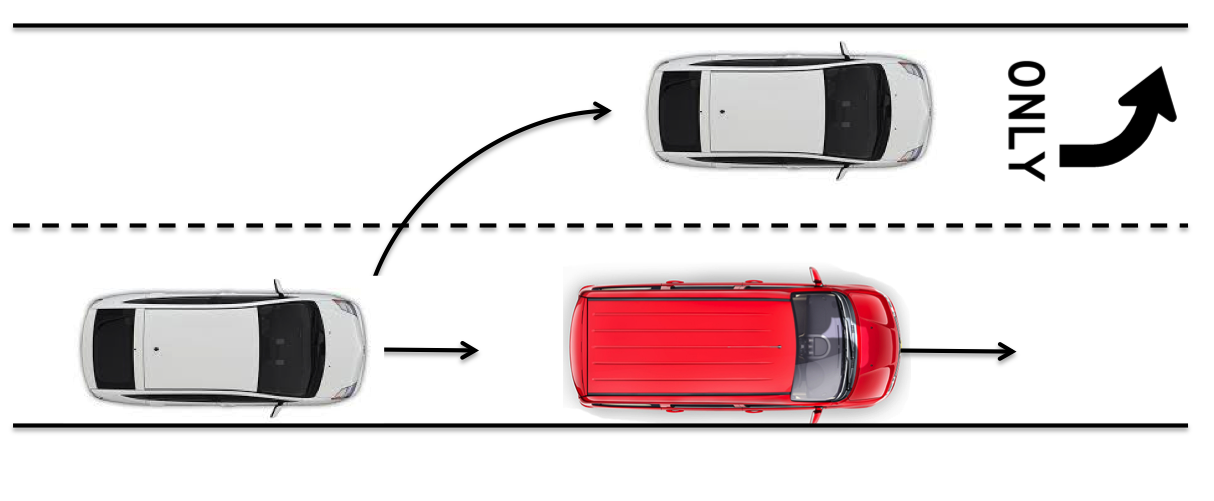
\includegraphics[scale=.4]{scenario.png}
	\caption{Pictorial description of target vehicle scenario}
\end{figure}
\subsection{Target Vehicle Model}
\subsubsection{Vehicle Dynamics}
Target vehicle plant has nonlinear dynamics described by bicycle model.
	\begin{equation}
	\begin{aligned}
	\ddot{\beta}=\left(\frac{C_rl_r-C_fl_f}{mv^2} \right)\dot{\psi}+\\
	\left(\frac{C_f}{mv} \right)\delta-\left(\frac{C_f+C_r}{mv} \right)\beta+y_{\beta}
	\end{aligned}
	\end{equation}
	\begin{equation}
	\begin{aligned}
	\ddot{\psi}=\left(\frac{C_rl_r-C_fl_f}{I_z} \right)\beta-\\
	\left(\frac{C_fl_f^2-C_rl_r^2}{I_z} \right)\left(\frac{\dot{\psi}}{v} \right)+
	\left(\frac{C_fl_f}{I_z} \right)\delta+y_{\dot{\psi}}
	\end{aligned}
	\end{equation}
	\begin{equation}
	\dot{v}=a_x+y_v
	\end{equation}
	\begin{equation}
	\dot{s_x}=v\cos{\beta+\psi}+y_{s_x}
	\end{equation}
	\begin{equation}
	\dot{s_y}=v\sin{\beta+\psi}+y_{s_y}
	\end{equation}
	\begin{equation}
	\dot{\delta}=v_w+y_d
	\end{equation}
	
	\(C_f,C_r\) and \(l_f, l_r\) describe respectively the cornering stiffness and distances from the center of gravity to the axles. \(I_z\) is the moment of inertia and \(m\) is the vehicle mass. \(\beta\) is the slip angle at the center of mass, \(\psi\) is the heading angle, \(\dot{\psi}\) is the yaw rate, \(v\) is the velocity, \(s_x\) and \(s_y\) are the x and y positions, and \(\delta\) is the angle of the front wheel. In the formulation of [6], the inputs to the system are \(a_x\), the logitudinal acceleration, and \(v_w\) the rotational speed of the steering angle. The \(y\) terms represent disturbances to the system. For example \(y_{\beta}\) and \(y_{\dot{\psi}}\) represent disturbances to the slip angle at the center of mass and the yaw rate. 
\subsubsection{Hybrid Model}
	\begin{enumerate}
	\item Trajectories are defined for right to left lane switch and left to right lane switch.
	\item Hybrid system modes are described by drive forward and lane change.
	\begin{enumerate}
		\item Lane change is hierarchical and has sub-modes, right to left, straight, and left to right.
		\item Each submode has same dynamics but implements a different motion primitive.
	\end{enumerate}

		\begin{figure}[tb]
			\label{fig:hybrid}
			\centering
			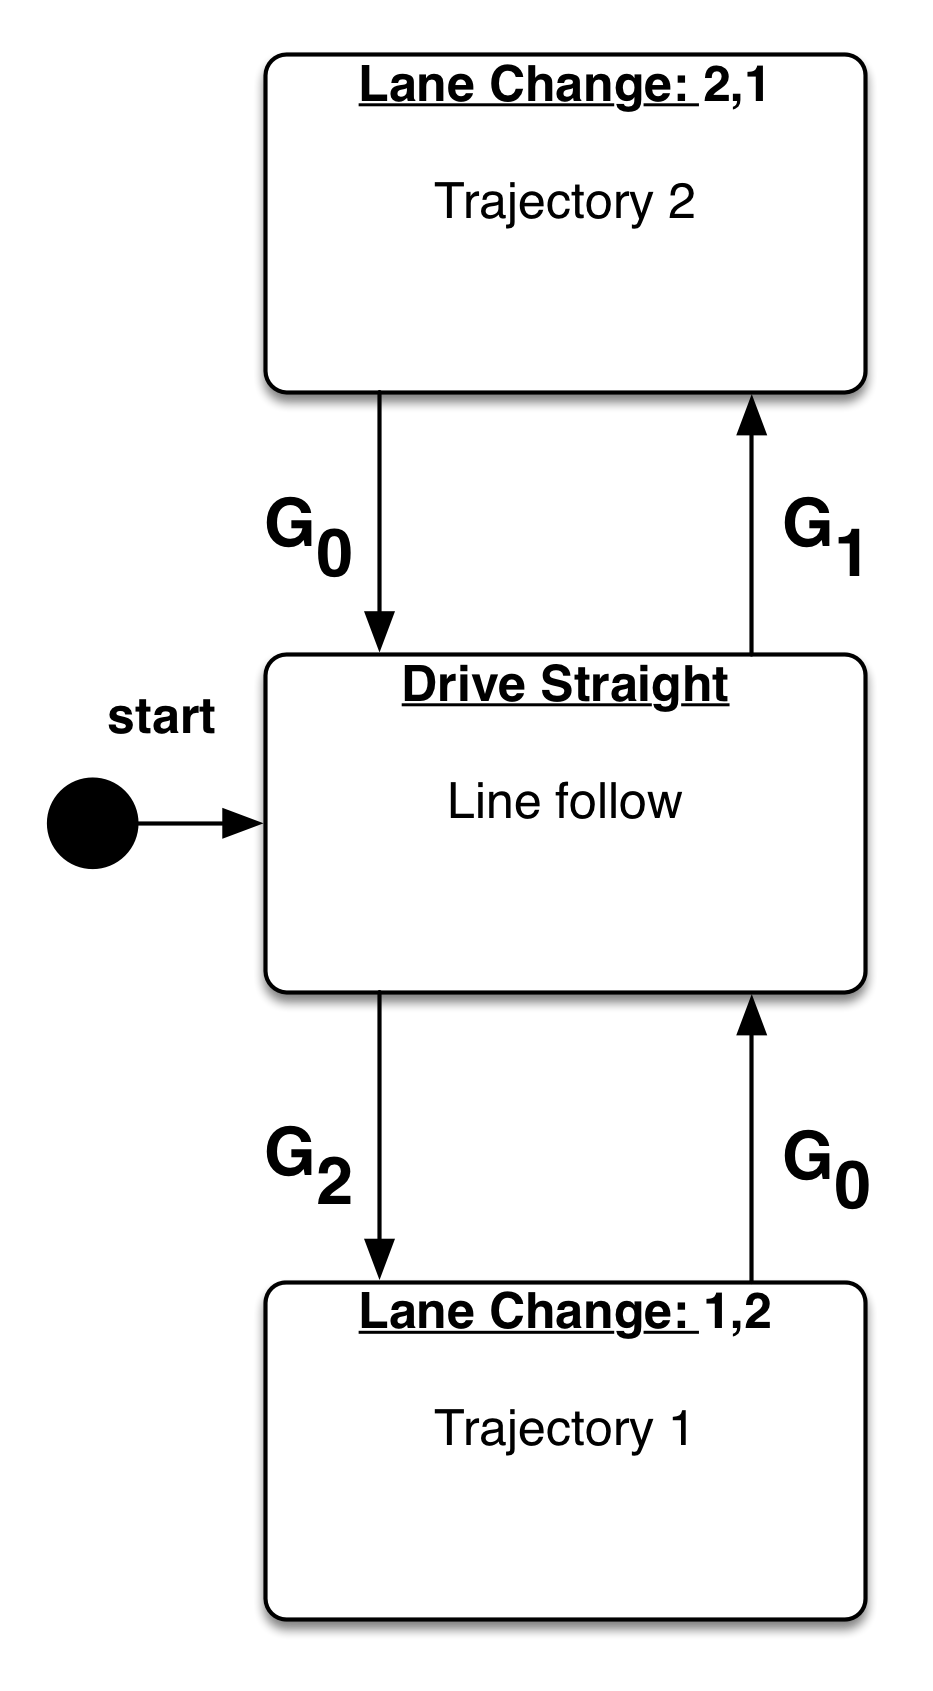
\includegraphics[scale=.5]{hybrid.png}
			\caption{Hybrid automata describing lane change}
		\end{figure}
	\item Fig.\ref{fig:hybrid} describes the system.
	\item[] \(G_1\) and \(G_2\) If there is a vehicle detected in the current lane traveling at a velocity less than the target vehicle's velocity, and there exists another lane which has the same direction of travel as the current lane, and the reachable set of the target vehicle executing a motion primitive for a lane change does not intersect with any other vehicle in the scenario, transition to the lane change mode.
	\item[] \(G_0\) If lane change motion primitive is complete, transition back to the follow lane mode.
		\end{enumerate}

\subsubsection{Plant Controller}
Final control equations generate inputs for the plant which represent longitudinal acceleration and the rate of change of the steering angle:
	\begin{equation}
	\begin{aligned}
	v_w=k_1(cos{(\Psi_d)}(s_{y,d}-s_y-w_y)\\
	-sin{(\Psi_d)}(s_{x,d}-s_x-w_x)\\ 
	+k_2(\Psi_d-\Psi-w_{\Psi}) \\
	+k_3(\dot{\Psi_d} -\dot{\Psi}-w_{\psi})\\
	-k_4(\delta-w_{\delta})
	\end{aligned}
	\end{equation}
	\begin{equation}
	\begin{aligned}
	a_x=k_5(cos{(\Psi_d)}(s_{x,d}-s_x-w_x)\\
	+sin{(\Psi_d)}(s_{y,d}-s_y-w_y)\\
	+k_6(v_d-v-w_v)
	\end{aligned}
	\end{equation}
ADD guard condition information


\subsection{Environmental Vehicle Model}
Environmental vehicle has simple 2D dynamics, no specific controller, non-determinism describes state evolution. When considering other agents (especially vehicles) in a scenario such non-linear dynamics are completely unnecessary. The primary reasoning is that the uncertainty about the state of other vehicles is not do to poor model parameter identification, but rather unknown inputs [2]. The dynamics of the other agents are described by equations (7) and (8) as in [3]:
\begin{equation}
\dot{s_x}=v\cos{\beta}
\end{equation}
\begin{equation}
\dot{s_y}=v\sin{\beta}
\end{equation}

\begin{enumerate}
	\item Environmental vehicle must drive forwards.
	\item Environmental vehicle must not change lanes if other lane is occupied.
	\item At every step the environmental vehicle can apply +/- some specified level of acceleration.
	\item At every step environmental vehicle can switch lanes if condition 2 is not violated.
\end{enumerate}
Environmental vehicle has simple 2D dynamics, no specific controller, non-determinism describes state evolution.
\begin{enumerate}
	\item Environmental vehicle must drive forwards.
	\item Environmental vehicle must not change lanes if other lane is occupied.
	\item At every step the environmental vehicle can apply +/- some specified level of acceleration.
	\item At every step environmental vehicle can switch lanes if condition 2 is not violated.
\end{enumerate}
\subsection{dReal Model}
\begin{enumerate}
	\item Consider several other vehicles in the environment with simple 2-D kinematics and the target vehicle with the nonlinear bicycle model dynamics. While in general the reachability problem for non-linear hybrid systems is undecidable. Recent work [1] has shown that if a user is able to specify a bound on the ODE which is an arbitrary positive rational number \(\delta\), then propositions in first order logic over a region \textit{unsafe} can be evaluated. Specifically a system, \(H\), is \(safe\) if it cannot reach \(unsafe\), and \(H\) is \(\delta-unsafe\) if \(H^d\) can reach \(unsafe\). 
\end{enumerate}
\subsection{Controller with Partial Dynamics}
A finite transition system describing the passing manuever is given in UPPAAL (or NuSMV).
\begin{figure}[tb]
	\label{fig:discreteview}
	\centering
	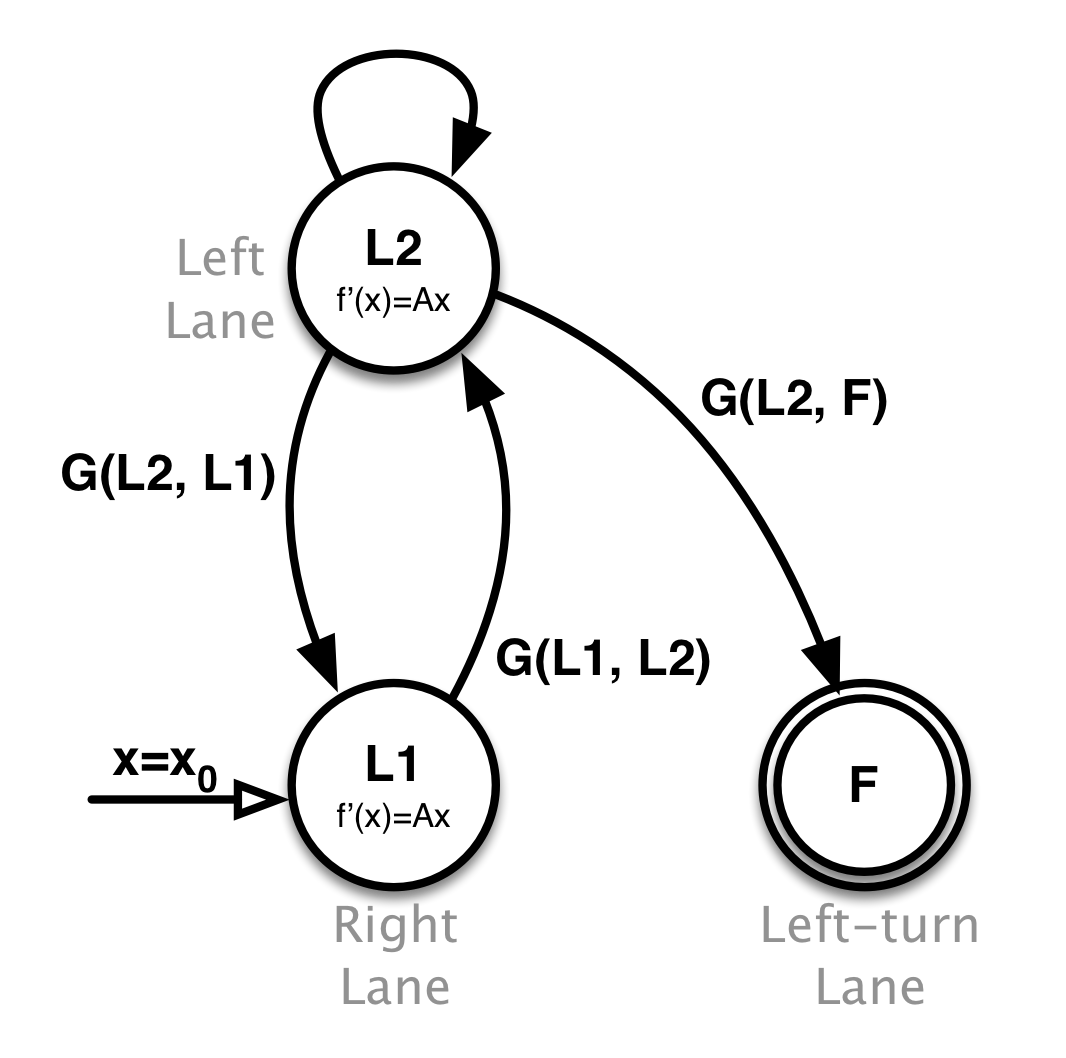
\includegraphics[scale=.7]{lane_change_timed.png}
	\caption{Automata with partial dynamics describing scenario}
\end{figure}